\documentclass[letterpaper,12pt]{article}
\usepackage[letterpaper]{geometry}
\usepackage[english]{babel}
\usepackage{empheq}
\usepackage{graphicx}
\usepackage{epstopdf}
\usepackage{listings}
\usepackage{color}
 
\definecolor{codegreen}{rgb}{0,0.6,0}
\definecolor{codegray}{rgb}{0.5,0.5,0.5}
\definecolor{codepurple}{rgb}{0.58,0,0.82}
\definecolor{backcolour}{rgb}{0.95,0.95,0.92}
 
\lstdefinestyle{mystyle}{
    backgroundcolor=\color{backcolour},   
    commentstyle=\color{codegreen},
    keywordstyle=\color{magenta},
    numberstyle=\tiny\color{codegray},
    stringstyle=\color{codepurple},
    basicstyle=\footnotesize,
    breakatwhitespace=false,         
    breaklines=true,                 
    captionpos=b,                    
    keepspaces=true,                 
    numbers=left,                    
    numbersep=5pt,                  
    showspaces=false,                
    showstringspaces=false,
    showtabs=false,                  
    tabsize=2
}
 
\lstset{style=mystyle}

\special{papersize=8.5in,11in}

\begin{document}

\begin{titlepage}
\newcommand{\HRule}{\rule{\linewidth}{0.5mm}} % Defines a new command for the horizontal lines, change thickness here

\center % Center everything on the page
%----------------------------------------------------------------------------------------
%	HEADING SECTIONS
%----------------------------------------------------------------------------------------

\textsc{\LARGE University of Hong Kong}\\[1.5cm] % Name of your university/college
\vspace{2.5cm}
\textsc{\Large COMP 3270 Artificial Intelligence }\\[0.5cm] % Major heading such as course name
\textsc{\large Fall term 2017}\\[0.5cm] % Minor heading such as course title

%----------------------------------------------------------------------------------------
%	TITLE SECTION
%----------------------------------------------------------------------------------------

\HRule \\[0.4cm]
{ \LARGE \bfseries Report of Mini Project - Othello}\\[0.4cm] % Title of your document
\HRule \\[1.5cm]
 
%----------------------------------------------------------------------------------------
%	AUTHOR SECTION
%----------------------------------------------------------------------------------------

\begin{minipage}{0.8\textwidth}
\begin{center} \large
\vspace{0.5cm}

Qiu Haoran \\ \vspace{0.3cm}\textsc{UID: 3035234478}\\
\vspace{2cm}
\end{center}
\end{minipage}

%----------------------------------------------------------------------------------------
%	DATE SECTION
%----------------------------------------------------------------------------------------

{\large 28/November/2017}\\[3cm] % Date - could also use \today

%----------------------------------------------------------------------------------------
%	LOGO SECTION
%----------------------------------------------------------------------------------------

%\includegraphics{Logo}\\[1cm] % Include a department/university logo - this will require the graphicx package
 
%----------------------------------------------------------------------------------------

\vfill % Fill the rest of the page with whitespace
\end{titlepage} 

\begin{abstract}
Othello, also named Reversi, is a strategy board game between two players. As an artificial intelligence game application, what a player is facing is an intelligence agent instead of another human. This report describes in detail about the AI methodology, such as the \textbf{search engine}, \textbf{$\alpha$-$\beta$ pruning}, \textbf{heuristics} applied, and the application \textbf{architecture}. Some other detail about the program like how \textbf{horizon effect} is avoided, the number of steps the AI looks ahead, and the precoded-database in use. In the end, instructions on how to deploy and run the game are given.
\end{abstract}

\section{Game Modeling}
\textbf{Initial State}: Initial game board is an 8 by 8 board with four disks placed in the center like the figure bellow.
\begin{figure}[!htb]
\centering
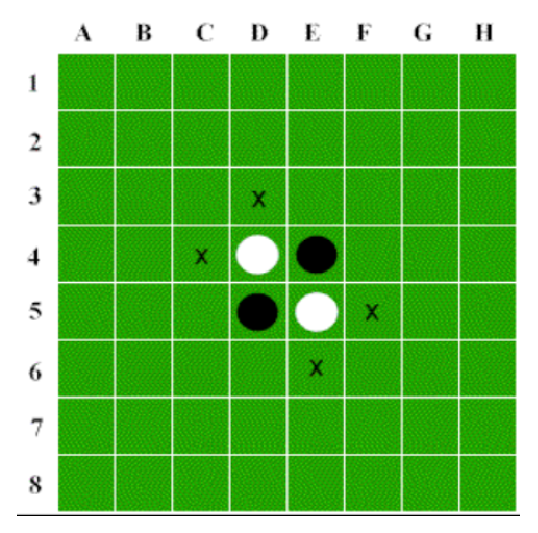
\includegraphics[scale=.6]{initial.eps}
\caption{Initial Board \& Possible Move}
\label{fig:digraph}
\end{figure}
\\
\noindent
\textbf{Players}: The game is a two-player game. One is the user, and the other is the computer. The player places black disks while the computer places white ones. The user (black) is the first to play and then two players place disks alternatively. If one of the two players does not have any legal moves, then this player pass his turn to the other player.
\\\\
\textbf{Actions}: Each player should place the disk to a position where the unplaced one can surround disk(s) with another same-color disk horizontally, vertically, or diagonally. In figure 1, the legal movements for the black are marked by cross signs.
\\\\
\textbf{Result(state,move)}: The transition model, which defines the result of a move.
\\\\
\textbf{Terminal Test}: The game is over when there's no legal move for both two players or the board is full.
\\\\
\textbf{Utility(state, player)}: A utility function defining a numerical value for the player at a particular state.
\\\\
The initial state, actions, and result(transition model) define the game tree for Othello - a tree where the nodes are game states and the edges are moves. It's also called a search tree is it's superimposed on the full game tree, and examines enough nodes to allow a player to determine what move to make.


\section{Artificial Intelligence Methodology}

\subsection{Minimax Search Algorithm with $\alpha$-$\beta$ Pruning}

The search method allows the agent to look ahead and explore different moves through a systematic generation of next possible moves. The heuristic function (elaborated in the next subsection) complements the search process by evaluating the state of the game along the various paths. The efficiency of the search technique determines the extent to which the game tree is explored. The greater the efficiency of the search technique, the greater the number of nodes that can be searched, hence the farther the agent could look ahead. An ideal search mechanism should be efficient and prune irrelevant paths without loss of any important information.\\\\
\noindent
Iterative-Deepening Minimax Search algorithm is used in this application with $\alpha$-$\beta$ Pruning. It becomes unclear as to the optimal depth to search up to, if the depth is to be defined
statically. Hence, we implemented alpha-beta with iterative deepening. The algorithm sets depth to a reasonable initial value of three. Then the depth is increased and the search is conducted
again. This is done till the timing constraints are not violated. Before searching with an increased depth, a naive check is made to ensure that the search about to be spawned will not violate timing constraints. Using the time taken for the previous depth, we approximately calculate a new depth at which the next iteration can take place. This new depth would be such that it finishes, according to the approximation, before the allotted time. If it doesn’t, the process is not preempted, and the execution exceeds by a few milliseconds. 

\subsection{Pseudo Code of the Algorithm}
\begin{lstlisting}
def search(board):
	depth = 2
	time_elapsed = 0
	initialize optimal_move to (-1, -1)
	optimal_board = board

	while time_elapsed < time_limit and still_have_to_dig:
		IDMinimax(board, 0, depth, 2, -infinity, infinity)
		update time_elapsed, optimal_board, optimal_move
		depth += 1
    
	return optimal_move

def IDMinimax(board, current_level, max_level, player, alpha, beta):
	if no_available_move or current_level == max_level:
    	return with flag "can_stop_dig"
	find successor boards
	if player is a maximizer:
		max_value = -infinity
		for each successor board:
		lookahead_board = IDMinimax(this_board, current_level+1, max_level, 3-player, alpha, beta)
		calculate the score for the board
		if the score > max_value:
			max_value = score
			best_board = this successor board
		alpha = max(alpha, score)
		if score > beta:
			return lookahead_board  # pruning happens here
	else if player is a minimizer:
		min_value = infinity
		for each successor board:
		lookahead_board = IDMinimax(this_board, current_level+1, max_level, 3-player, alpha, beta)
		calculate the score for the board
		if the score < min_value:
			min_value = score
			best_board = this successor board
		beta = min(beta, score)
		if score < alpha:
			return lookahead_board  # pruning happens here
	return best_board
\end{lstlisting}

\subsection{Evaluation Function - Heuristics Applied}

Due to the limitation of resources, a computer cannot store and evaluate all possible states. Aligning to the utility function, evaluation function is used for giving agent heuristics about a middle state. Based on the rules and strategies, assign scores for the leaves of the tree, the evaluation function is:

\begin{center}
$Score(move(row, col)) = P(move(row, col)) + C(move(row, col)) + L(move(row, col)) + M(move(row, col)) + S(move(row, col))$
\end{center}
\noindent
The following examples is made for the agent (i.e. white).

\begin{itemize}
\item \textbf{Piece Difference} $P(move(row, col))$: measure how many pieces of each color on the board. Let $B$ and $W$ represent the human player and the agent. If $W > B$, then score is $W/(B+W) * 100$; if $W < B$, then score is $-B/(B+W) * 100$; If $W = B$, then score is 0.
\item \textbf{Corner Captions} $C(move(row, col))$: measures how many corners are owned by each player. Let $B$ and $W$ be the number of black and white tiles in the corners, then the score is $25*(W - B)$.
\item \textbf{Corner Closeness} $L(move(row, col))$: measures the pieces adjacent to empty corners. Let $B$ and $W$ be the number of black and white tiles that are adjacent to empty corners, respectively, then the score is $12.5*(W - B)$.
\item \textbf{Mobility} $M(move(row, col))$: measures how many legal moves each player has. Let $B$ and $W$ be the number of all possible legal moves black and white players could make. If $W > B$, then score is $W/(B+W) * 100$; if $W < B$, then score is $-B/(B+W) * 100$; If $W = B$, then score is 0.
\item \textbf{Stability} $M(move(row, col))$: Stability of coins is a key factor in Othello. The stability measure of a coin is a quantitative representation of how vulnerable it is to being flanked. The more stable pieces a state contains, the higher the score will be. Assign 1 for a stable piece, 0 for a semi-stable piece, -1 for an unstable piece.
\end{itemize}

\subsection{Others}

After running a few experiments with a time limit set to three seconds. The experiments were run with the optimal weights. The average depth searched was 5.6, and the maximum time taken for any search
was 2.75 seconds. The time taken for an average move was 2.69 seconds.\\\\
\noindent
We have a database of predetermined moves, which we refer to when possible. This avoids any time wasted in  searching when the next move to make is an obvious one. For example, if a corner could be captured, then that should be the next move executed, hence searching would be redundant in such cases.

\section{Program Architecture}

The program application uses PyGame as its game engine. The whole flow is then divided into three layers. The first layer is the game engine, which the second layer, i.e. the game logic, is based on. The third layer is the implementation of Artificial Intelligence algorithms, which can be accessed by the second layer.

\subsection{View Layer - Why PyGame?}
The pygame library is an open-source module for the Python programming language specifically intended to help programmers make games and other multimedia applications. Built on top of the highly portable SDL (Simple DirectMedia Layer) development library, pygame can run across many platforms and operating systems.\\
\begin{figure}[!htb]
\centering
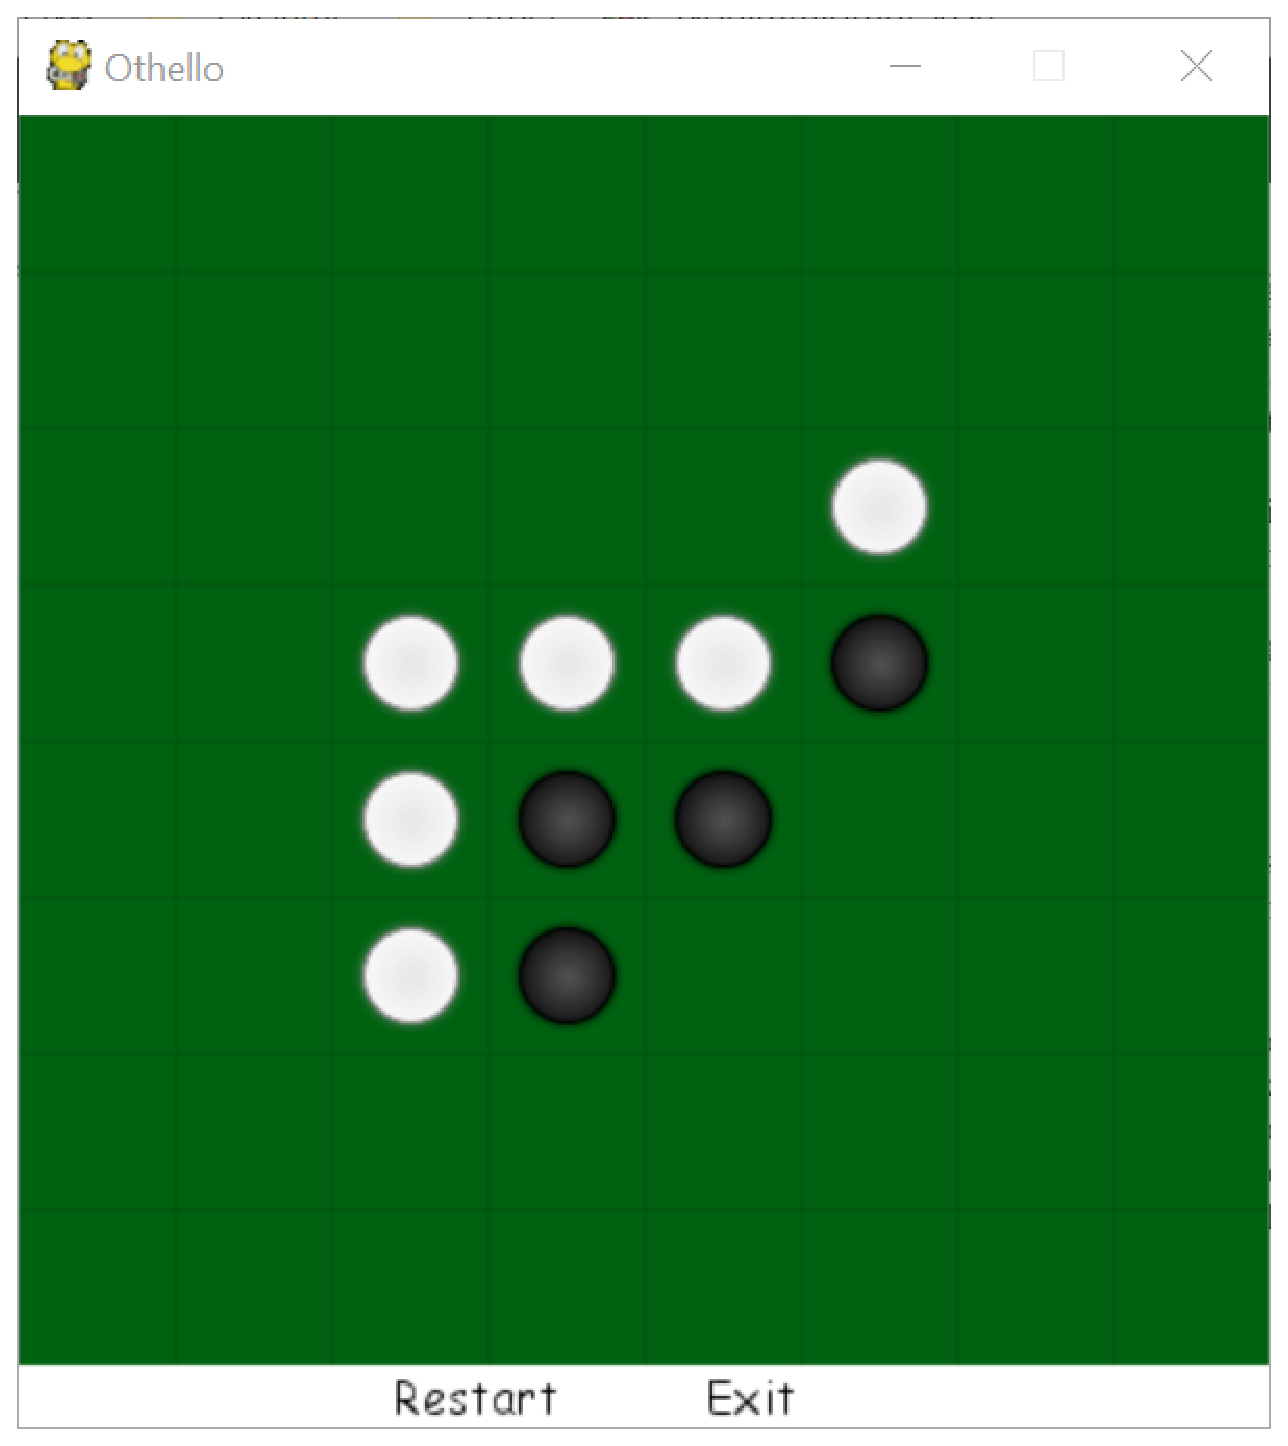
\includegraphics[scale=.3]{GUI.eps}
\caption{Graphical Interface of Othello}
%\label{fig2:digraph}
\end{figure}\\
\noindent
By using the pygame module, programmers can control the logic and graphics of their games without worrying about the backend complexities required for working with video and audio.
\noindent
The GUI is an 8 by 8 board with black and white pieces. Two buttons are set at the bottom of the window. Player could restart or exit the game by pressing the corresponding button. Each move can be controlled by the mouse.

\subsection{Model \& Control Layer - Game Flow}
Module "othello" with class "Othello" implements the game flow. Attribute "useAI" determines whether AI could be used or not. If the attribute is set to false, then this is a two-player Othello, otherwise, this is a computer-player Othello.\\\\
\noindent
Attribute "player" determines who is holding the turn, 1 (black) represents the player 1, and 2 (white) represents player 2 or the AI. Before the player click a block, the model will first check whether there's available movement. If there is, then the player could move. If it's a valid move, then flipping of the pieces will be performed, otherwise, the player could see there's no change in the board, i.e. he or she should give a valid move and then the other player (AI) could move.\\\\
\noindent
If two players cannot move, game over.

\section{Instructions on How to Run the Application}

In Windows,

\begin{itemize}
\item Install python 3 (3.6.1 or above)
\item Install pygame \texttt{py -m pip install pygame}
\item Go to the root directory and run \texttt{py main.py}
\end{itemize}

\noindent
In Linux,

\begin{itemize}
\item Check python version: \texttt{python3 --version}
\item If not installed: \texttt{sudo apt-get install python3.6}
\item Install pygame: \texttt{sudo apt-get install python3-pygame}
\item Go to the root directory and run \texttt{python3 main.py}
\end{itemize}

\noindent
If there's any problem on running the application, please feel free to contact with James.Qiu by email: jamesqiu@hku.hk.


\begin{thebibliography}{}
\bibitem{}
Reversi, Wikipedia, September 2017, $https://en.wikipedia.org/wiki/Reversi$
\bibitem{}
Getting Started with PyGame. Retrieved from \\$https://www.pygame.org/wiki/GettingStarted\#Pygame Installation$
\bibitem{}
An Analysis of Heuristics in Othello, University of Washington. Retrieved from \\$https://courses.cs.washington.edu/courses/cse573/04au/Project/mini1/RUSSIA/Final_Paper.pdf$
\bibitem{}
Artificial Intelligence: A Modern Approach, S. Russell \& P. Norving, 2016, Retrieved from $http://aima.cs.berkeley.edu/$
\end{thebibliography}
\end{document}